\documentclass[10pt,letterpaper,onecolumn]{article}
\usepackage{amsmath}
\usepackage{graphicx} 
\usepackage{hyperref}
\usepackage{subfig}
\graphicspath{ {img/} }
\begin{document}
\title{Observation of Compton Scattering via Cs-137 source and Aluminum rod}
\author{
 Akhil Deshpande \\*
 Nirmal Patel \\*
 \\*
 PHY 474 Advanced Laboratory \\*
 Spring 2024 \\*
 Dr. Deepa Thomas \\*
 Department of Physics \\*
 The University of Texas at Austin \\*
 Austin, TX 78712, USA
}
\date{\today}
\maketitle
\begin{abstract}
    This report presents the findings of an experiment designed to observe Compton scattering using a Cs-137 source and an aluminum rod. The objective was to empirically verify the Compton effect, which predicts a shift in photon wavelength upon scattering by electrons, indicative of the particle nature of light. Through calibration using Cs-137 and Ba-133 sources, we converted MCA bin numbers to photon energies, enabling measurement of the Compton shift at various scattering angles. The experimental data was fitted against the theoretical predictions made by the Compton formula and further corroborated by the Klein-Nishina formula to account for relativistic effects. The results yielded a coefficient of determination (\(R^2\)) of 0.969, demonstrating a high correlation between observed and predicted values and affirming the validity of the Compton and Klein-Nishina models.
\end{abstract}
\section{Introduction}
\subsection{Historical Context}
According the theory of classical electromagnetism, the wavelength of a scattered ray should be equivalent to the wavelength of the incident ray. This phenomenon is described by the theory of Thomson scattering. In 1923, Arthur Compton observed a different effect. Compton an instance in which when a high energy photon interacts with a charged particle, it releases valence electrons from the outer shell of the particle. More formally, Compton scattering is a type of scattering that is caused by the interactions between particles and waves in the X-ray to gamma ray range. 


Energies from waves in this spectrum will usually be lower than their incident energies. This correlates to an increase in their wavelength. The amount this wavelength changes is called the Compton shift. This occurs after a relativistic, high energy photon ineracts inelastically with the charged particle. This results in an energy shift from the photon to the particle, and therefore a loss of energy exhibited by the photon.\cite{Pattison1975}
\begin{figure}
    \begin{center}
        \includegraphics*[width=3.5in]{scattering.jpg}
        \caption{This image depicts the Compton effect. An incoming X-ray is shown to have an inelastic collision with an electron, losing some of its energy. Image taken from Encyclopedia Brittanica \cite{ComptonEffectImage}.}
    \end{center}
\end{figure}
\section{Theoretical Background}
The Compton shift can be explained as a formula that is dependent on the angle of scattering \cite{PhysRev.21.483}:
\begin{equation}
    \label{comptonShiftWavelength} 
    \lambda' = \lambda + \frac{h}{m_e c}(1 - cos(\theta)),
\end{equation}
where 
\begin{itemize}
\item $\lambda'$ represents the wavelength after scattering, 
\item $\lambda$ represents the wavelength before scattering, 
\item $h$ is Planck's constant,
\item $m_e$ is the rest mass of the electron,
\item $c$ is the speed of light, and
\item $\theta$ is the angle of scattering.
\end{itemize}
This formula can also be expressed in terms of photon energy:
\begin{equation}
    \label{comptonShiftEnergy} 
    E_{\gamma'} = \frac{E_{\gamma}}{1 + \left( {E_{\gamma}}/{m_e c^2} \right)(1 - \cos(\theta))},
\end{equation}
where 
\begin{itemize}
\item $ E_{\gamma'}$ represents the final state photon energy, and
\item $E_{\gamma}$ represents the initial energy, 
\end{itemize}
and all other variables are as mentioned above
\cite{Taylor2004ModernPhysics}.


These two equations are the basis for this experiment.
The Klein-Nishina formula also provides a description to account for relativistic and quantum effects in Compton scenarios


The significance of the Klein-Nishina formula lies in its ability to accurately predict the differential cross section for the scattering of photons by free electrons, as given by:

\begin{equation}
\frac{d\sigma}{d\Omega} = \frac{1}{2} r_0^2 \left( \frac{E_{\gamma'}}{E_{\gamma}} \right)^2 \left( \frac{E_{\gamma'}}{E_{\gamma}} + \frac{E_{\gamma}}{E_{\gamma'}} - \sin^2 \theta \right),
\end{equation}
\\
where

\begin{itemize}
    \item  $r_0$ is the classical electron radius, 
    \item $E_{\gamma}$ is the initial photon energy, 
    \item $E_{\gamma'}$ is the energy after scattering, and
    \item  $\theta$ is the scattering angle.
    \end{itemize}   
which describes the energy \( E_{\gamma'} \) of the scattered photon as a function of the incident photon energy \( E_{\gamma} \), the electron rest mass \( m_e \), the speed of light \( c \), and the scattering angle \( \theta \).


The Klein-Nishina formula is crucial for the correct interpretation of Compton scattering results, particularly in high-energy physics and astrophysics, where photon energies approach or exceed the rest mass energy of the electron, \( m_e c^2 \). It has also been instrumental in confirming the dual wave-particle nature of light, serving as a cornerstone in the development of quantum electrodynamics.

\section{Experimental Procedure}
\subsection{Apparatus}
\subsubsection*{Radioactive Source}
Due to the necessity of a high-energy photon source, we used a sample of Cs-137 as a radioactive gamma source. This source was fitted into a lead ball with a 1 centimeter hole drilled through the center of it. There were several lead blocks placed in front of this hole, each with the same 1 centimeter hole drilled through them. To align the source with our detector, we used a laser to ensure that the 1 centimeter hole was in like with the center of the scintillator detector. 
\subsubsection*{Scintillator}
Our scintillator was a Sodium Iodide Scintillator manufactured by Saint-Gobain. A NaI (sodium iodide) scintillator operates on the principle of scintillation, where incident gamma rays interact with the crystal lattice to produce visible light. In the context of Compton scattering, when high-energy photons collide with the electrons in the NaI crystal, part of the photon's energy is transferred to the electron, leading to the ejection of the electron and the photon's energy reduction. This process results in the excitation of atoms within the NaI crystal, which de-excite by emitting photons in the visible spectrum. These emitted photons are then detected by an adjacent photomultiplier tube (PMT), converting the light into an electrical signal proportional to the energy of the incident gamma rays. This mechanism is crucial for Compton scattering experiments, as it allows for the precise measurement of energy distributions of scattered photons, providing insights into the scattering process and the interaction of gamma rays with matter.
\subsubsection*{ORTEC Components}
We also utilized an ORTEC power supply, MCA, and a spectroscopy amplifier. The power supply was an ORTEC 556 set to 1000 Volts. This powered the ORTEC preamiplifier connected to the scintillator. The scintillator fed data to the ORTEC 672 spectroscopy amplifier. This amplifier had a shaping time of 1, an input of positive polarity on normal mode, a BLR rate of high, and a triangle shaping. This module output data to our ORTEC 927 MCA, which sorted our signals into discrete channels that correspond to the energy of the gamma rays.
\begin{figure}
    \begin{center}
        \subfloat[\centering The spectroscopy amplifier]{{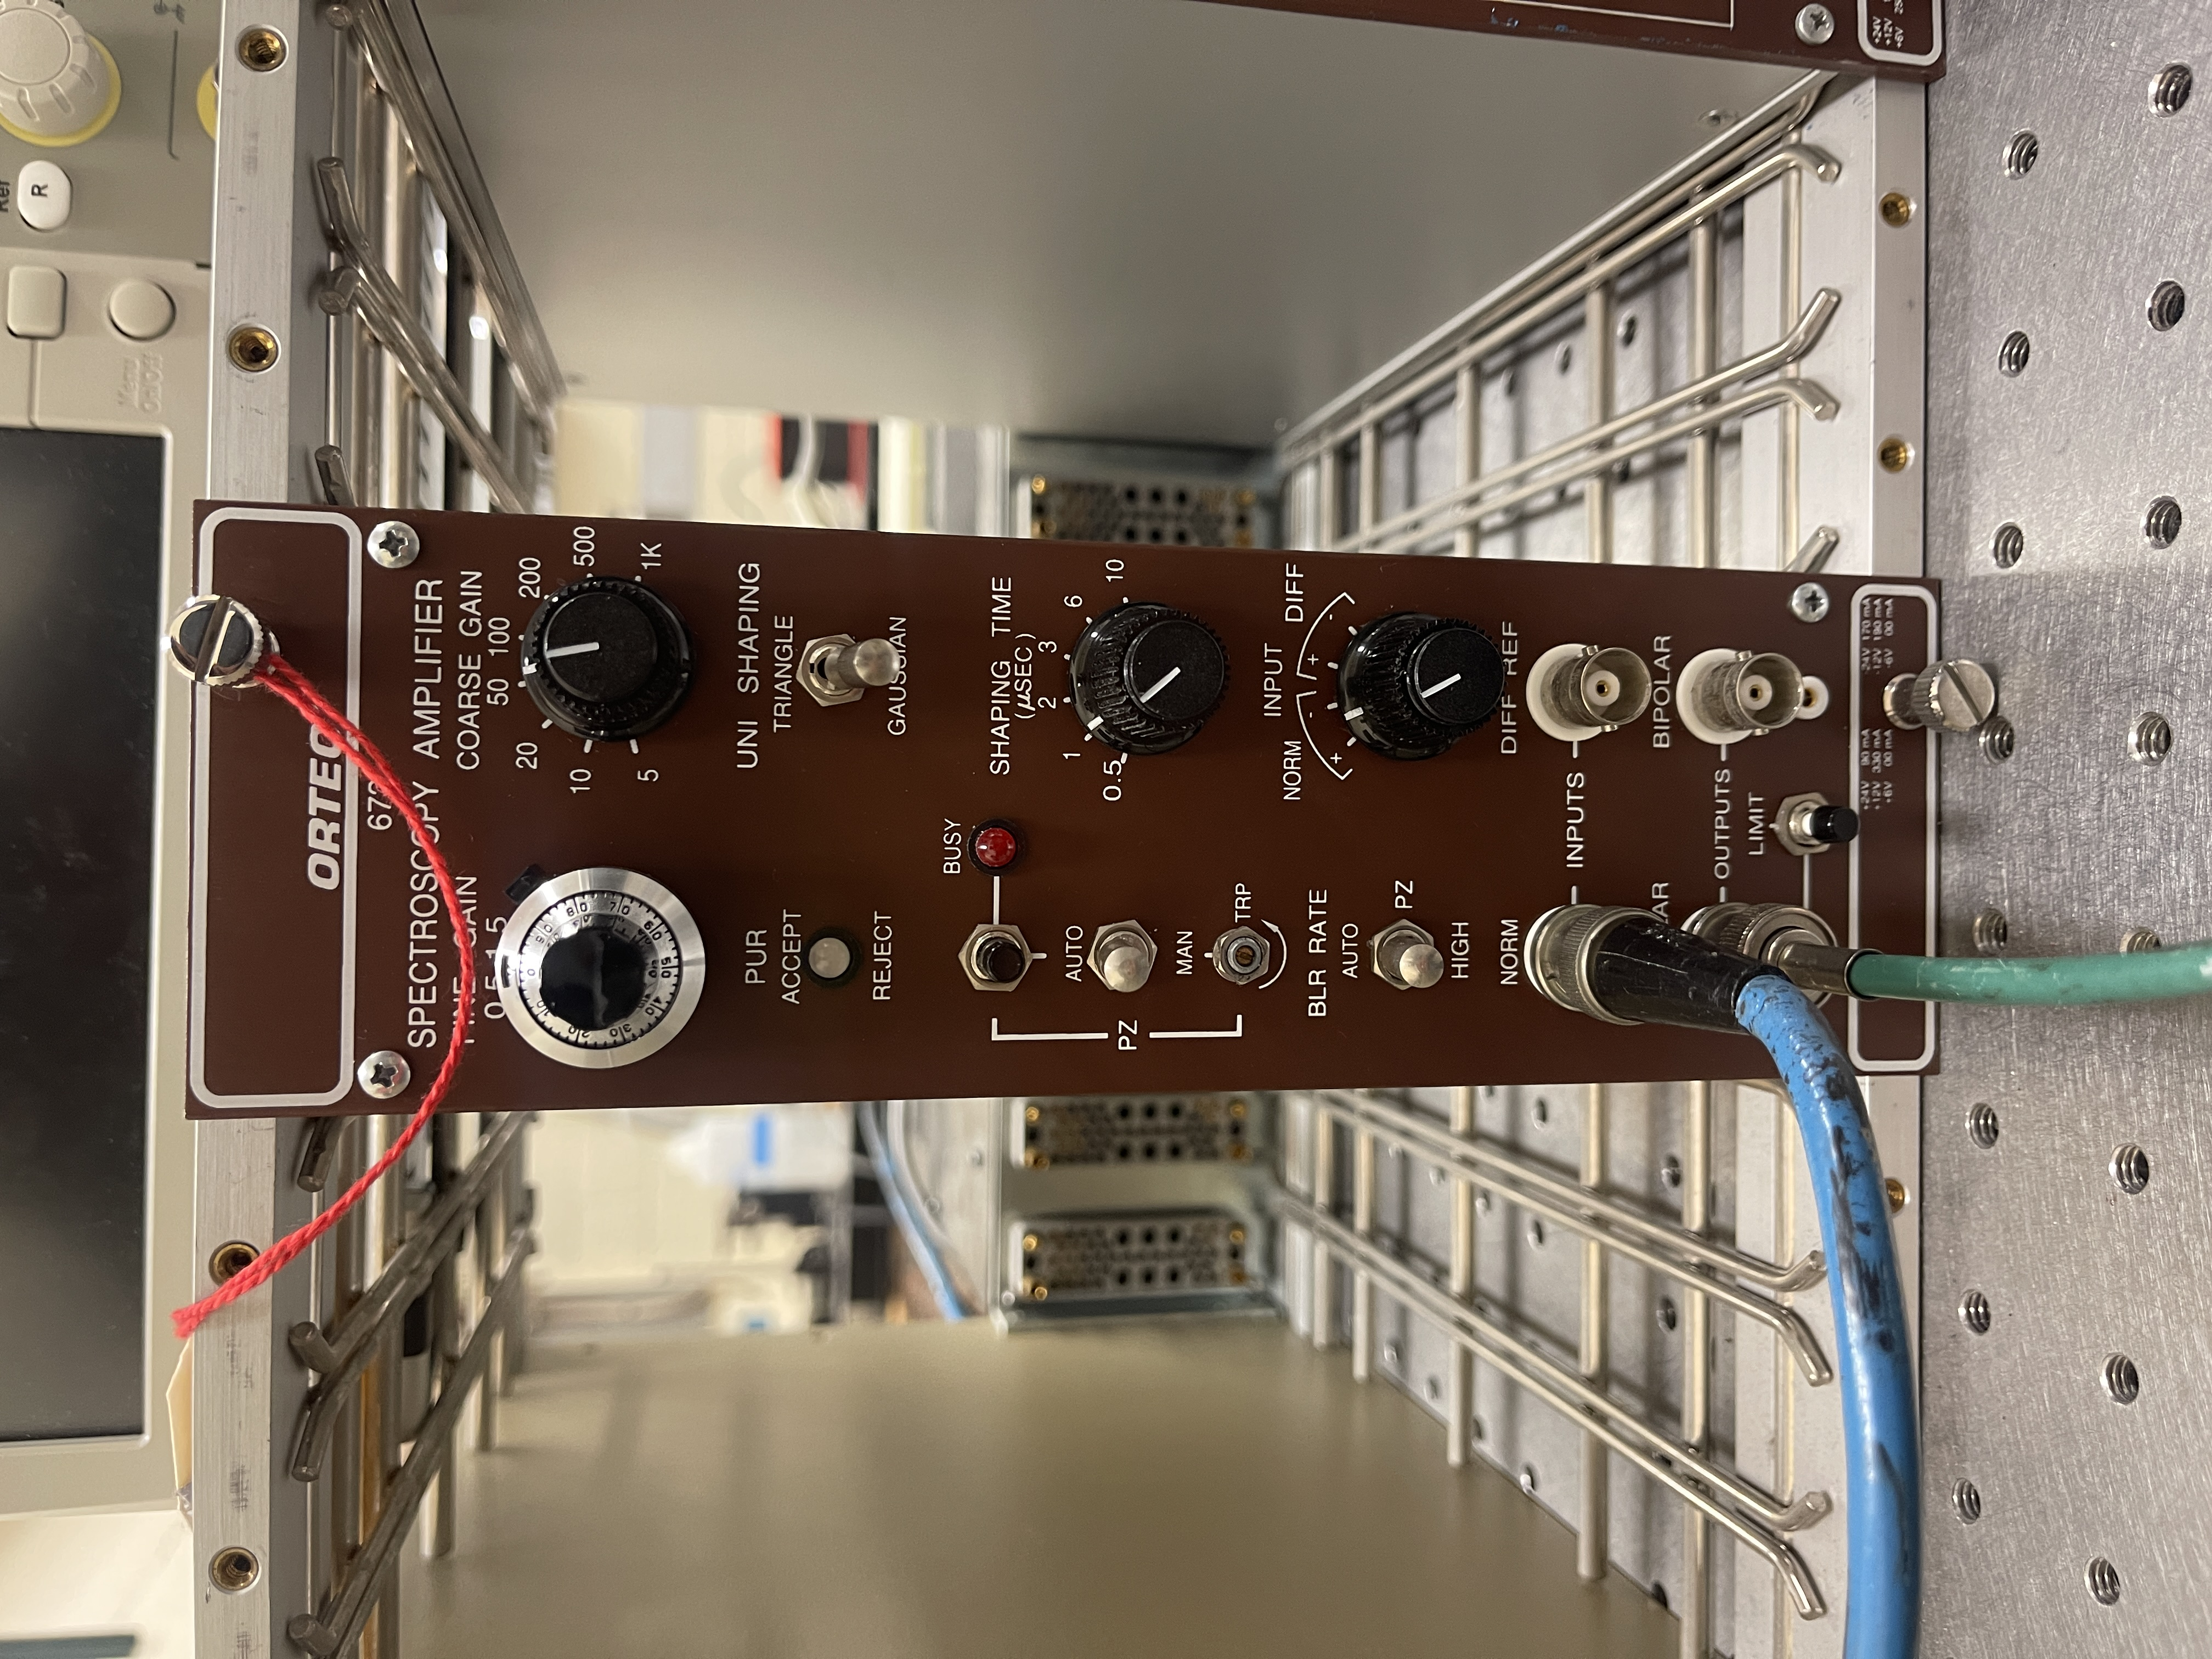
\includegraphics[width=6cm, angle = 270]{spectroscopyamplifier.JPG}}}%
        \qquad
        \subfloat[\centering The MCA and power supply]{{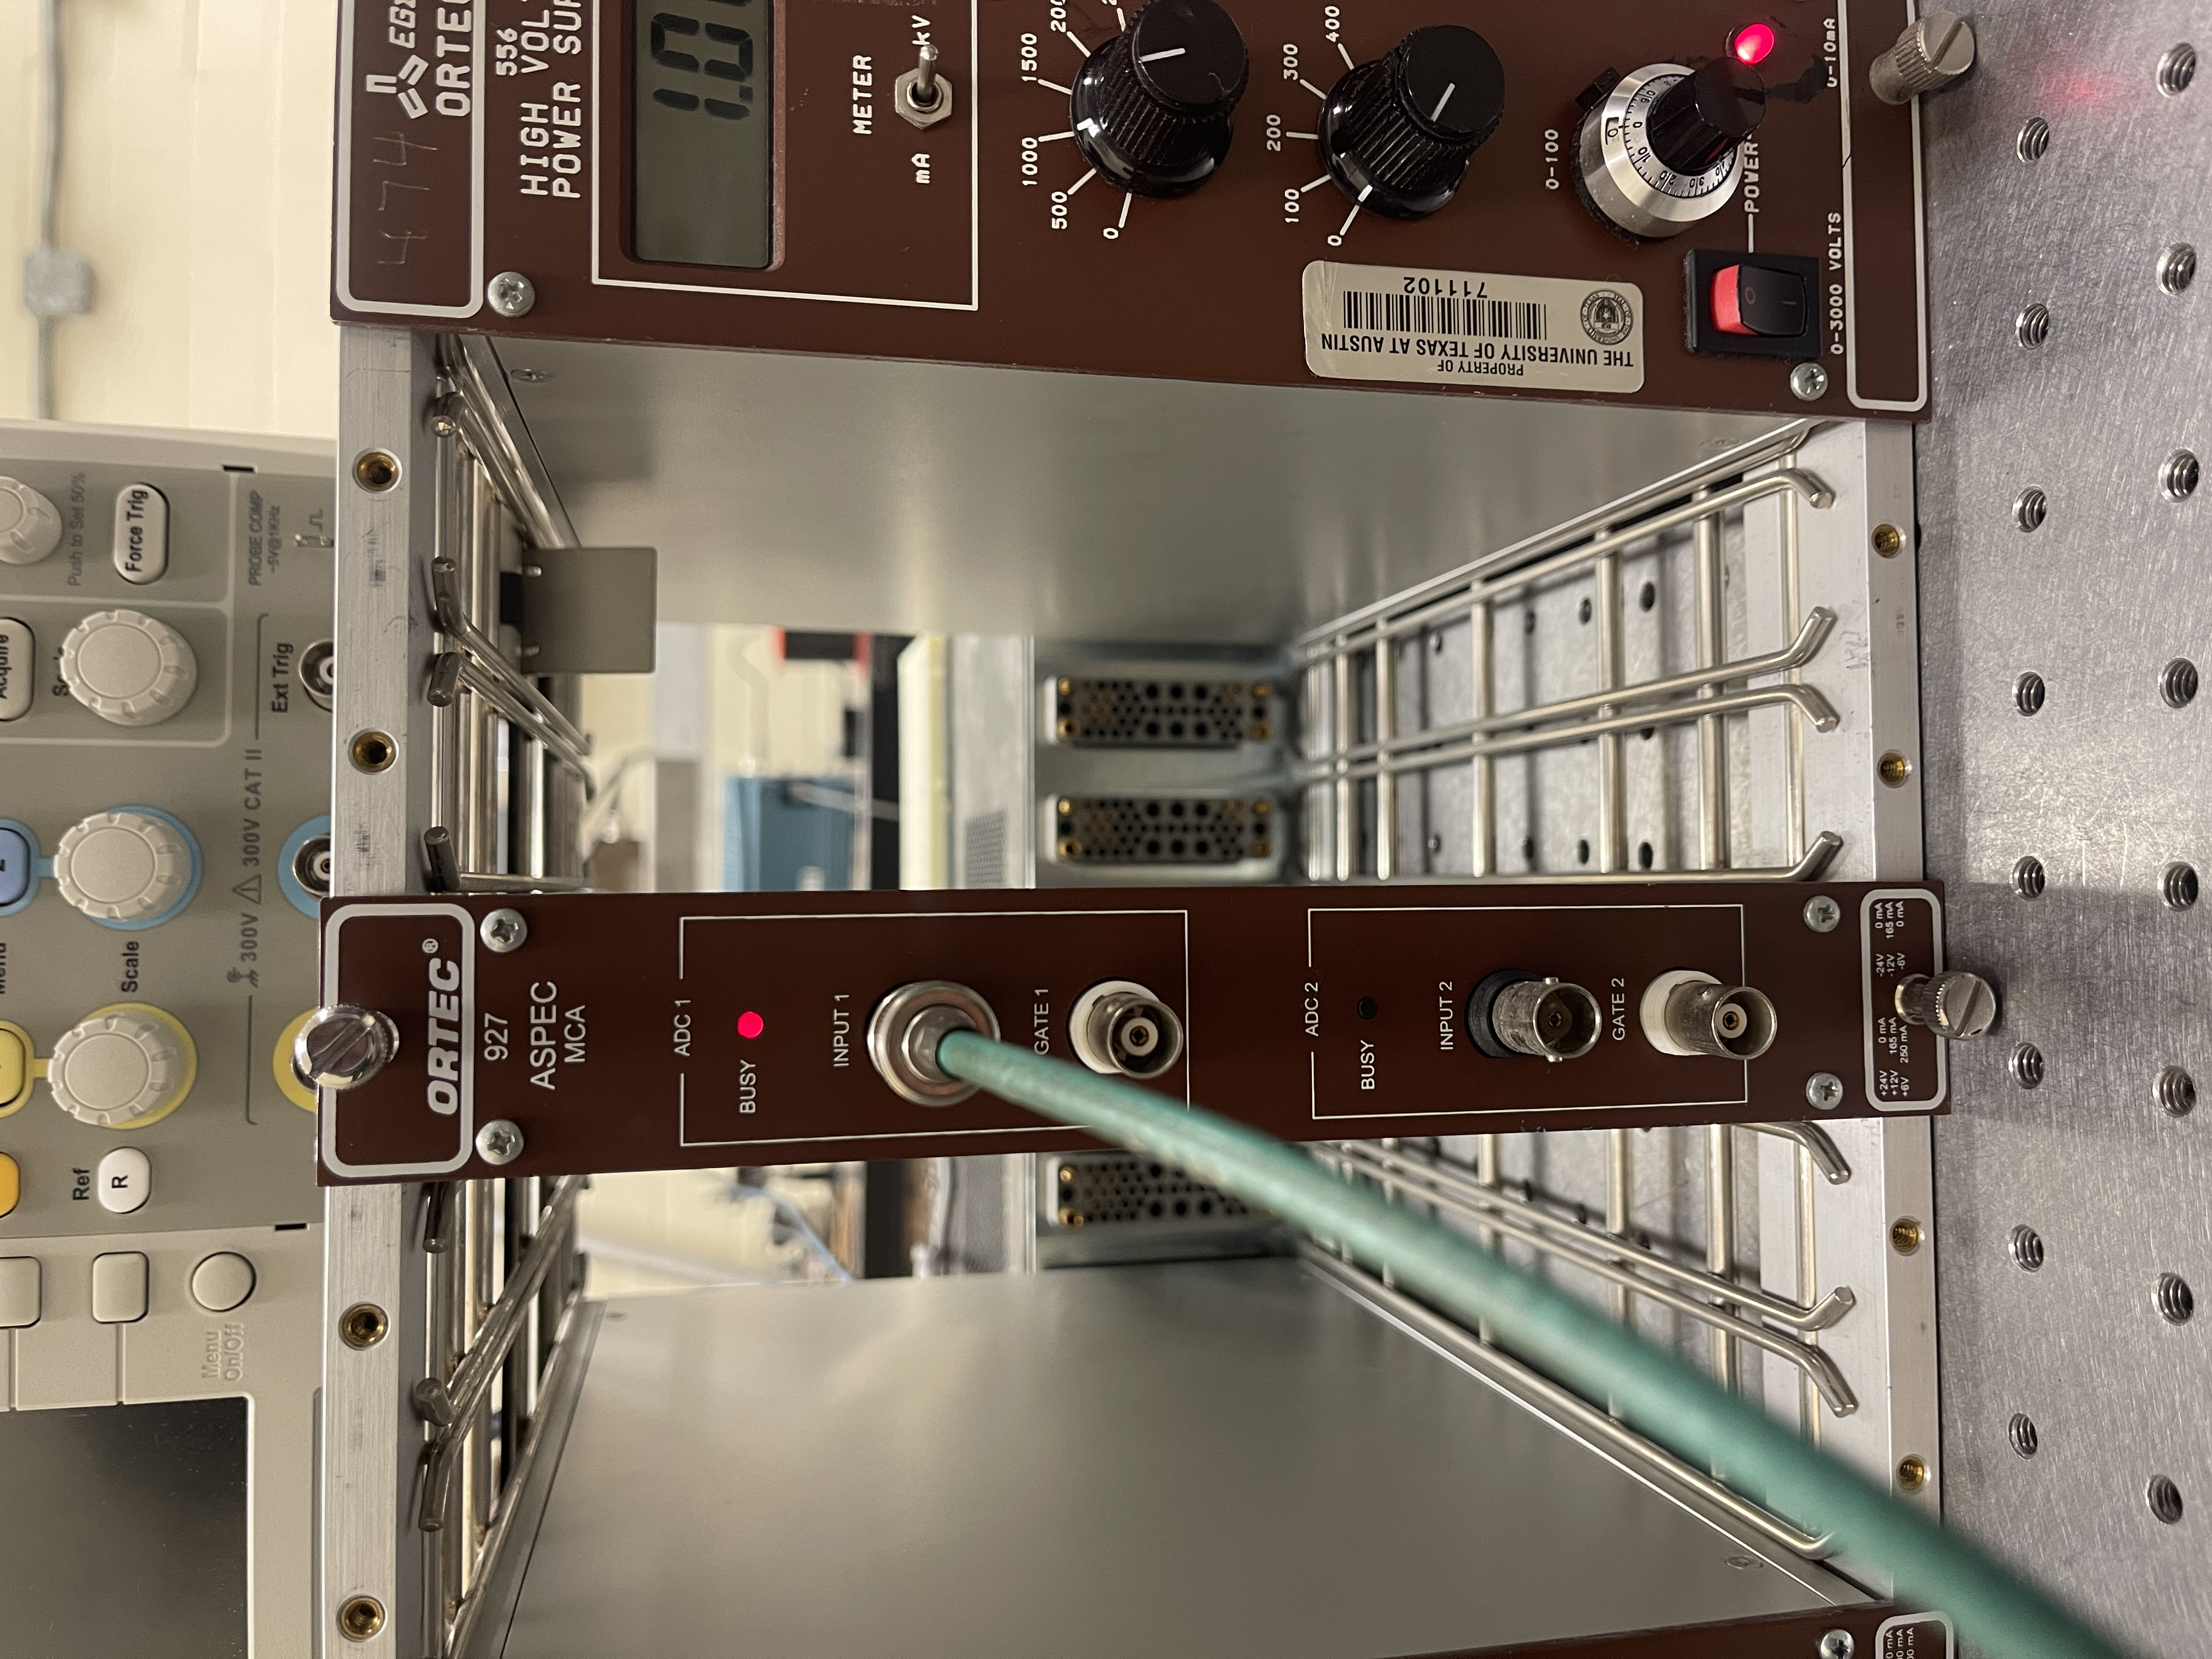
\includegraphics[width=6cm, angle = 270]{mca.JPG} }}%
        \caption{Here, we have the spectroscopy amplifier, shown on the right, and the MCA and power supply shown on the left. The settings for each are as described in the ORTEC Components subsection. For clarification, the power supply is set to 1 kV, or 1000 V.}%
        \label{fig:apparatus}%
    \end{center}
\end{figure}
\subsubsection*{Computer Software}
We then ran trials on the lab computer's MAESTRO software. This software output data as .chn files which we used Python3 to analyze. All code and analysis functions can be found on \href{https://github.com/adeshpande03/seniorlab}{my personal github}. Furthermore, in order to make data collection easier, we created .job files which MAESTRO used to automatically save our files in case the computer turned off after being on for long periods of time. These are also found on my github.
\subsection{Data Collection}
Before we began collecting data, we collected some calibration data. To do so, we taped a button source of Cs-137 to the scintillator. We then took data for ten minutes using this button source in order to observe a calibration spectrum for Cs-137. This was important as the MCA sorts the data into 'bins' which have no real significance in the real world. In order to convert these bins to their corresponding photon energies, we need to assign each bin number an energy level, which we do using an established source. As our experimental radioactive source was Cs-137, we thought it fitting to use a Cs-137 button source for precision. 


We also took some optional calibration data using Ba-133. This Ba-133 data was collected in much the same way that the Cs-137 button source was. We taped a button source of Ba-133 to the scintillator, and collected data based on the resulting spectrum. We were able to observe a well-established peak on the spectrum, and compared this to the accepted value of the spectroscopy peak. For these reasons, the calculations involving the correlations of the bins to the energies of the photons were done using both spectra, instead of just the Cs-137 source.


We collected our data using MAESTRO and .job files. First, we set the scattering angle on a rotating stage. Then, we edited our .job file to reflect the amount of time, in seconds, we wanted to record data for. We then turned on the power supply and let the apparatus capture data for the set time. We did this twice per angle. Once for a run with the .5" Alumimun rod, to measure the actual scattering, and once without, to measure the background radiation of the room. This procedure was done once per angle from 0 degrees to 80 degrees, as that was the furthest the stage would rotate.


We collected data for equivalent time intervals for each angle. For example. we collected data at 80 degrees with the rod for 24 hours, and also without the rod for 24 hours. This was done in order to have a consistent number of counts for each angle measurement. 

\begin{table}[tbp]
    \centering
    \begin{tabular}{ll}
    Angle                    & Time (seconds)             \\ \hline
    \multicolumn{1}{|l|}{0}  & \multicolumn{1}{l|}{3600}  \\ \hline
    \multicolumn{1}{|l|}{10} & \multicolumn{1}{l|}{3600}  \\ \hline
    \multicolumn{1}{|l|}{20} & \multicolumn{1}{l|}{3600}  \\ \hline
    \multicolumn{1}{|l|}{30} & \multicolumn{1}{l|}{10800} \\ \hline
    \multicolumn{1}{|l|}{40} & \multicolumn{1}{l|}{64800} \\ \hline
    \multicolumn{1}{|l|}{50} & \multicolumn{1}{l|}{64800} \\ \hline
    \multicolumn{1}{|l|}{60} & \multicolumn{1}{l|}{64800} \\ \hline
    \multicolumn{1}{|l|}{70} & \multicolumn{1}{l|}{64800} \\ \hline
    \multicolumn{1}{|l|}{80} & \multicolumn{1}{l|}{86400} \\ \hline
    \end{tabular}
\end{table}
\begin{figure}
    \caption{A table depicting the time intervals we used for our data. Each time is entered in seconds, and each angle was run twice -- once for a background run, and once to measure the scattering.}
\end{figure}
\subsection{Data Analysis}
\subsubsection*{Calibration}
Our data analysis began with writing code to associate each bin with an energy level using the peaks we measured for the Ba-133 and Cs-137 buttons sources. We did so by finding the peak of each graph, and fitting the bin to an accepted energy value for each peak. In the case of the Cs-137 sample, this was at the 662keV mark\cite{GammaSpectacularCS137}. In the case of the Ba-133 sample, this was at the 356keV mark \cite{GammaSpectacularBA133}. Figure \ref{fig:calibration} shows this data. 
\begin{figure}[hbt!]
    \begin{center}
        {{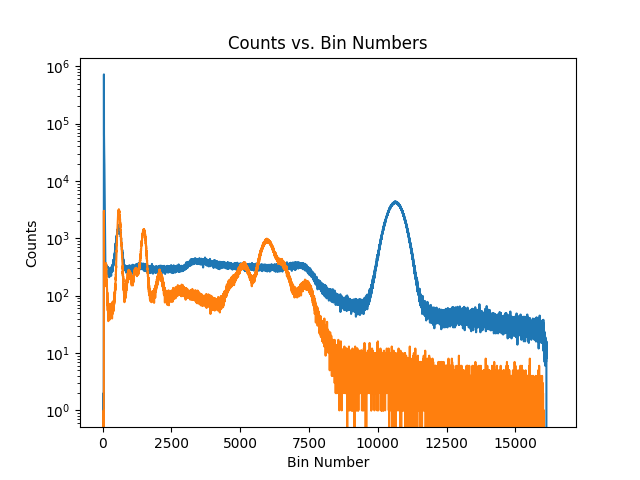
\includegraphics[width=7cm]{calib.png} }}%
        \caption{A graph depicting the calibration data we used to correlate bins to energies. The y-axis represents the number of counts, while the x-axis represents the bin number. The blue spectrum represents the Cs-137 source, while the orange spectrum represents the Ba-133 source. We would expect to see a distinct peak on each spectrum, which we do. For the Cs-137 spectrum, we see a peak around the 11000 bin mark, while for the Ba-133, we see a peak around the 6500 bin mark.}%
        \label{fig:calibration}%
    \end{center}
\end{figure}
\subsubsection*{Angular Data Analysis}
When analyzing data, we had two sets of files -- one set that contained the data for the runs with the rod and one that contained the background data. In order to get meaningful data from the scattering trials, we converted each data set into numpy arrays of size 16384 and subtracted each bin between the two trials. We used sizes of 16384 as this was the same size as the dataset, and also the same number of bins we used in MAESTRO when recording. This method allowed us to minimize the processing of data before analysis. We were then left with data that clearly showed where the peaks occurred. We loaded this data into a python program, and used a curve fitting algorithm to calculate exactly where the peaks in the data were. Furthermore, in order to minimize error, we restricted the domain of the curve fitting algorithm to an acceptable radius around the peak. We did this by visual cues, looking at the graphs and seeing where the most relevant peaks were, further estimating by theoretical calculations.

\begin{figure}[hbt!]
    \begin{center}
        {{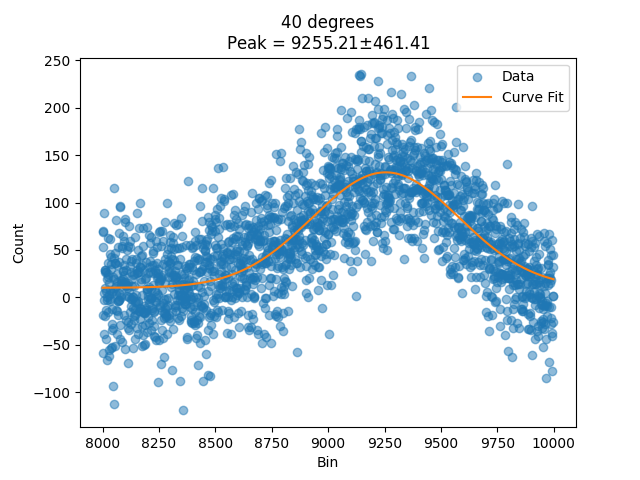
\includegraphics[width=7cm]{40.png} }}%
        \caption{A graph depicting our data for the 40 degree measurement we took. The y-axis represents the amount of counts, while the x-axis represents the bin number. We can clearly see the fitted peak of the graph, shown to be the value on the graph.}%
        \label{fig:40}%
    \end{center}
\end{figure}

Once we found out how each bin correlated to an energy, we began by fitting each data set to a peak-finding algorithm. Figure \ref{fig:40} is an example of one of our angular data sets, as well as the curve fit that was applied to analyze where the peak in the image was. 

As we got closer to the 80 degree mark, we ran into some Compton effects. As a result, our peak became less clear, and we had to manually restrict the data set more. For example, in the 40 degree analysis, we analyzed the dataset from bins 8,000 to 10,000. This was a range of about 2,000 bins, which allowed us to see a very clear peak with an extremely low error margin. Figure \ref{fig:80} shows us that when we were selecting the bins to analyze in the 80 degree measurement, we only let the program analyze 600 bins, as we had to visually select where the peak occurred. This method of selectively analyzing the domain, similar to the calibration calculation, let us minimize the uncertainty in the peak measurement. 

\begin{figure}[hbt!]
    \begin{center}
        {{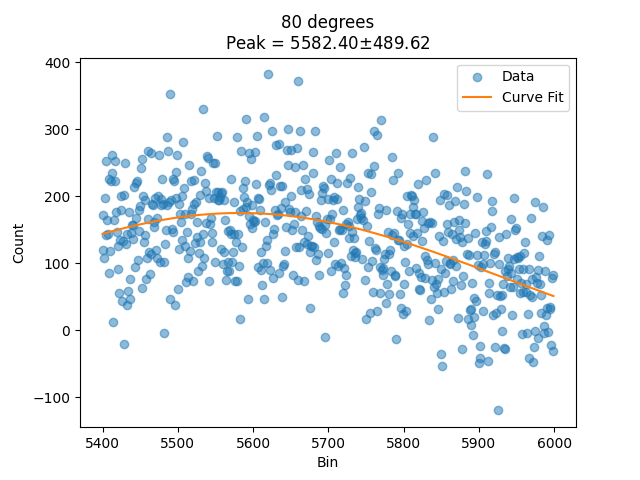
\includegraphics[width=7cm]{80.png} }}%
        \caption{A graph depicting our data for the 80 degree measurement we took. The y-axis represents the amount of counts, while the x-axis represents the bin number. We see the range of analysis was only 600 bins here as we ran into Compton effects when analyzing on a higher scale.}%
        \label{fig:80}%
    \end{center}
\end{figure}


\subsubsection*{Compton Scattering Fit}
Once the peak was calculated for each angle, we fit these peaks to the Compton formula. We did so by mapping the theoretical function data against our real data, and seeing how well the fit matched. This is shown in Figure \ref{fig:comfit}. In this figure, we can clearly see that the blue points (our experimental data) match the theoretical data. 

\begin{figure}[hbt!]
    \begin{center}
        {{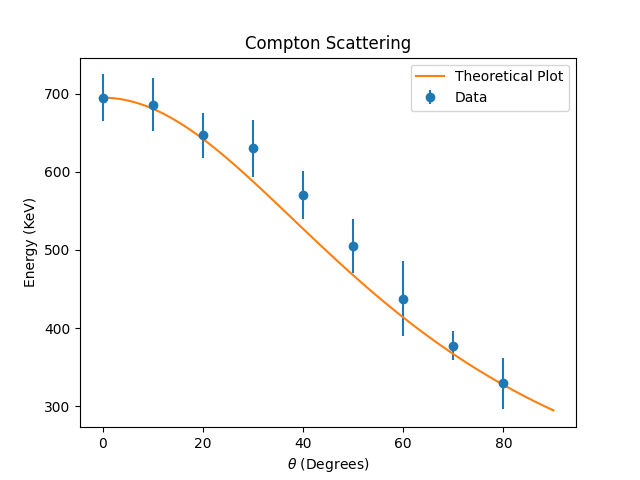
\includegraphics[width=7cm]{ScatteringFit.png} }}%
        \caption{A graph depicting our data for the Compton scattering fit. We have Energy with units of kiloelectron volts plotted on the y-axis, and our degrees on the x-axis. Each point corresponds to a separate trial at a distinct angle. We should see the blue points match the orange line, as this would represent an accurate correlation in our data.}%
        \label{fig:comfit}%
    \end{center}
\end{figure}

Then, to quantify the correlation between our experimental data and the theoretical data, we modeled the $R^{2}$ value of our data. We did this by modeling our $E(0)/E(\theta)$ versus our $1 - cos(\theta)$ data. We then used a least squares regression to generate our $R^{2}$ value. Figure \ref{fig:r2} shows that our $R^{2}$ data was 0.969. This means that our data indicates a high level of explanatory power of the regression model. Specifically, it suggests that approximately 96.9\% of the variance in the dependent variable can be predicted from the independent variable(s). This high \(R^2\) value generally implies a strong fit between the model and the observed data, indicating that the model can explain most of the variability in the response variable with its predictions.


\begin{figure}[hbt!]
    \begin{center}
        {{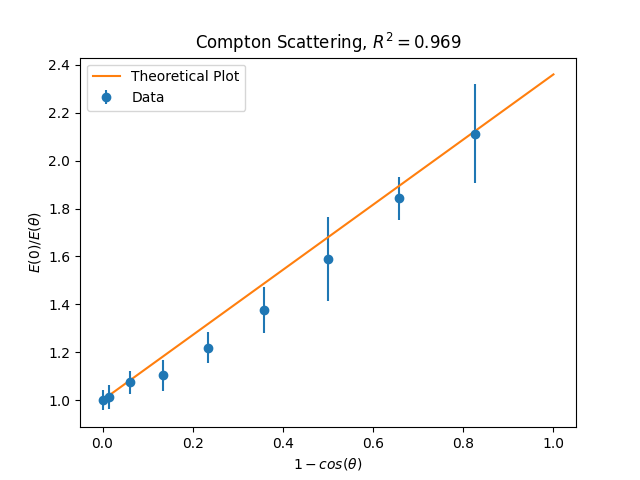
\includegraphics[width=7cm]{R2Compton.png} }}%
        \caption{A graph depicting our data for the Compton scattering fit. This data models our $E(0)/E(\theta)$ data versus our $1 - cos(\theta)$ data. We expect to see the blue dots line up with the theoretical data, as this would represent a good fit for our data.}%
        \label{fig:r2}%
    \end{center}
\end{figure}

\subsubsection*{Klein-Nishima Formula}
Finally, we plotted our results against the Klein-Nishima formula. We did so in a similar way to our Compton fits. In order to compare the Klein-Nishima formula to the classical model of electrodynamics, we also plotted the Thomson model to show the validity of the Klein-Nishima formula. Figure \ref{fig:kn} shows this relation. Our experimental data closely matches the Klein-Nishima formula in this case, while showing that the Thomson model does not hold true on this scale.
\begin{figure}[hbt!]
    \begin{center}
        {{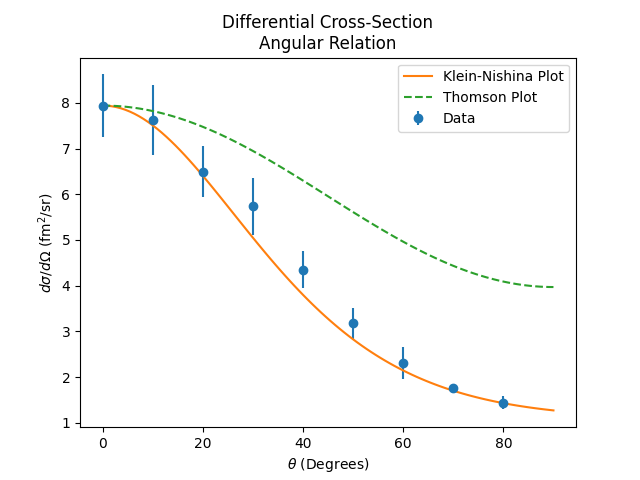
\includegraphics[width=7cm]{KNvsT.png} }}%
        \caption{A graph depicting our data for the Klein-Nishima fit. The y-axis represents the differential cross section, while the x-axis represents our angle. Each angle corresponds to a trial we conducted. The Klein-Nishima formula, depicted in orange, closely matches our experimental data. Furthermore, the Thomson model of classical electrodynamics strays quickly from our experimental data.}%
        \label{fig:kn}%
    \end{center}
\end{figure}

\subsection*{Error and Uncertainty}
This experiment had a few sources of error. The primary source of error in this experiment most probably came from background radiation. While we did subtract out the background radiation from each trial, there is a high probability that the trials with the aluminum rod suffered from some sort of noise error. Furthermore, the counts are subject to couting errors, as well as errors in the strength of the radiation source. Compared to lab reports from previous years, the radiation source was appro 7.5 millicuries in 2010. As Cs-137 has a half life of about 30 years, this means that today, in 2024, the sample probably decayed around 25\% of what it was in 2010. This would result in us getting lower counts and gamma ray emissions than those in previous experiments done here in Advanced Laboratory. 

Other sources of error could be the settings on our ORTEC machines. We followed advice from previous lab reports stating that the optimal voltage on the power supply was 1000 volts, and copied many of the other settings from those years as well. Errors could have easily been generated by propogating across the years, meaning that if we changed the settings on the power supply, preamiplifier, or spectroscopy amplifier, we may have been able to mitigate some sources of error that appeared in our results.

\section{Results and Conclusions}
\subsection*{Results}
The experiment successfully demonstrated Compton scattering, with the observed data closely matching theoretical predictions based on the Compton formula and the Klein-Nishina formula. The calibration process using Cs-137 and Ba-133 sources provided a reliable method for converting MCA bin numbers to photon energies, which was crucial for analyzing the scattering data.

The angular data analysis revealed clear peaks corresponding to scattered photon energies at various angles, from which the Compton shift was calculated. The fit of experimental data to the Compton formula yielded an \(R^2\) value of 0.969, indicating a high degree of correlation (96.9\%) between the observed data and the theoretical model. This strong fit suggests that the experiment accurately captured the dynamics of Compton scattering, with the experimental setup effectively demonstrating the energy and wavelength shift predicted by Compton's theory.

\subsection*{Conclusion}
The high \(R^2\) value achieved in this experiment underscores the precision and reliability of the experimental design and execution. The data's strong alignment with theoretical predictions confirms the Compton effect's significance in understanding photon-electron interactions and the quantum nature of light. This experiment not only reinforces the principles behind Compton scattering but also highlights the utility of the Klein-Nishina formula in describing the scattering process at higher energies, where relativistic effects become significant.

In conclusion, this experiment offers compelling evidence for the Compton effect. The methodologies employed, from calibration to data analysis, provide a robust framework for exploring complex phenomena in the laboratory setting.


\paragraph*{Acknowledgments}
I would like to thank my lab partner, Nirmal Patel for his assistance on data collection. Furthermore, I'd like to thank Dr. Deepa Thomas, and Dr. Matthew Dwyer for their assistance throughout the measurement and set up processes. 
\newpage
\bibliographystyle{plain} 
\bibliography{refs} 

\end{document}

